\documentclass[oneside,final,14pt]{extreport}
\usepackage{pdfpages} % поддержка вставки страниц из pdf-файлов
\usepackage[onehalfspacing]{setspace} % 1,5 интервал
\usepackage[top=2.0cm,bottom=2.0cm,left=2.0cm,right=1.0cm]{geometry} % поля
\usepackage{lscape} % поддержка альбомной ориентации страниц
\usepackage{indentfirst} % красная строка
\setlength\parindent{1.5cm} % установка величины отступа красной строки

% Шрифты
\usepackage[cm-default]{fontspec}
\usepackage{xunicode}
\usepackage{xltxtra}
%\setromanfont[Mapping=tex-text]{Times New Roman}
\setmainfont[Mapping=tex-text]{Times New Roman}
\setsansfont{Calibri}
\setmonofont{Consolas}
\defaultfontfeatures{Scale=MatchLowercase, Mapping=tex-text} % одинаковый рост строчных букв у разных гарнитур, маппинги TeXовских лигатур вроде -- и ---
\usepackage{ulem} % поддержка подчёркиваний

% Поддержка русского языка и русскоязычных стилей
\usepackage{polyglossia}
\setmainlanguage[babelshorthands=true]{russian} % основной язык - русский
\setotherlanguage[variant=us]{english} % дополнительный язык - английский

%\usepackage{amsmath}
% Формулы
\usepackage{amstext} % поддержка кириллицы в математических формулах
\usepackage{amssymb} % дополнительные символы в математических формулах
\usepackage{chngcntr} % управление нумерацией
\counterwithout{equation}{chapter} % сквозная нумерация формул

% Формат заголовков
\usepackage{titlesec}
\newcommand{\nhspacesize}{10pt}
\titleformat{\chapter}[hang]{\righthyphenmin62\sloppy\Large\bfseries}{\thechapter}{\nhspacesize}{} % righthypenmin62 - не переносить слова в названиях глав
\titleformat{\section}[hang]{\sloppy\large\bfseries}{\thesection}{\nhspacesize}{}
\titleformat{\subsection}[hang]{\sloppy\normalsize\bfseries}{\thesubsection}{\nhspacesize}{}
\titlespacing*{\chapter}{\parindent}{-30pt}{*4}
\titlespacing*{\section}{\parindent}{*1}{*2}
\titlespacing*{\subsection}{\parindent}{*1}{*1}

% Формат списков
\usepackage{enumitem}
\setlist{nolistsep} % убрать лишний интервал между элементами списка
\setlist[itemize,1]{label={–}, labelindent=\parindent, leftmargin=*} % маркированные списки: символ - короткое тире, выравнивание символа по красной строке
\AddEnumerateCounter{\asbuk}{\asbuk}{д} % последний параметр - самый широкий символ в перечислении
\setlist[enumerate,1]{label={\asbuk*}), labelindent=\parindent, leftmargin=*}
\setlist[enumerate,2]{label={\arabic*}), leftmargin=\parindent}

% Поддержка изображений
\usepackage{graphicx}
\graphicspath{{./images/chapter1/}{./images/chapter2/}{./images/chapter3/}{./images/chapter4/}} % пути к каталогам с изображениями
\usepackage{svg} % поддержка вставки векторных (SVG) изображений (из Inkscape) - команда includesvg

% Красивые таблицы
\usepackage{makecell}
\usepackage{multirow}

% Формат рисунков и таблиц
\usepackage{caption} % подписи
\captionsetup{labelsep=endash, textformat=simple, figurename=Рисунок, tablename=Таблица, figurewithin=none, tablewithin=none} % разделитель подписи и названия - короткое тире, заголовок - название float'a и номер, имена рисунков и таблиц по ГОСТу, сквозная нумерация рисунков и таблиц
\captionsetup[figure]{position=above}
\captionsetup[table]{singlelinecheck=false, position=top, justification=raggedright}
% подписи многостраничных таблиц
\DeclareCaptionLabelFormat{continued}{#1~#2 (\textit{продолжение})}
\captionsetup[ContinuedFloat]{labelformat=continued}
\usepackage{floatrow} % пакет для настройки размещения float'ов и их подписей
\floatsetup[table]{style=plaintop, justification=justified} % название над таблицей, таблица выровнена по ширине влево

% Библиография и библиографические ссылки
\usepackage{cite}
% Замена формата нумерации списка литературы с "[1]" на "1."
\makeatletter
\renewcommand{\@biblabel}[1]{#1.}
\makeatother
\bibliographystyle{utf8gost705u}
\gappto\captionsrussian{\renewcommand{\bibname}{Список использованных источников}}

% Оглавление
\gappto\captionsrussian{\renewcommand{\contentsname}{Содержание}}
\usepackage[subfigure,titles]{tocloft}
\renewcommand{\cftchapleader}{\bfseries\cftdotfill{\cftdotsep}}

\begin{document}
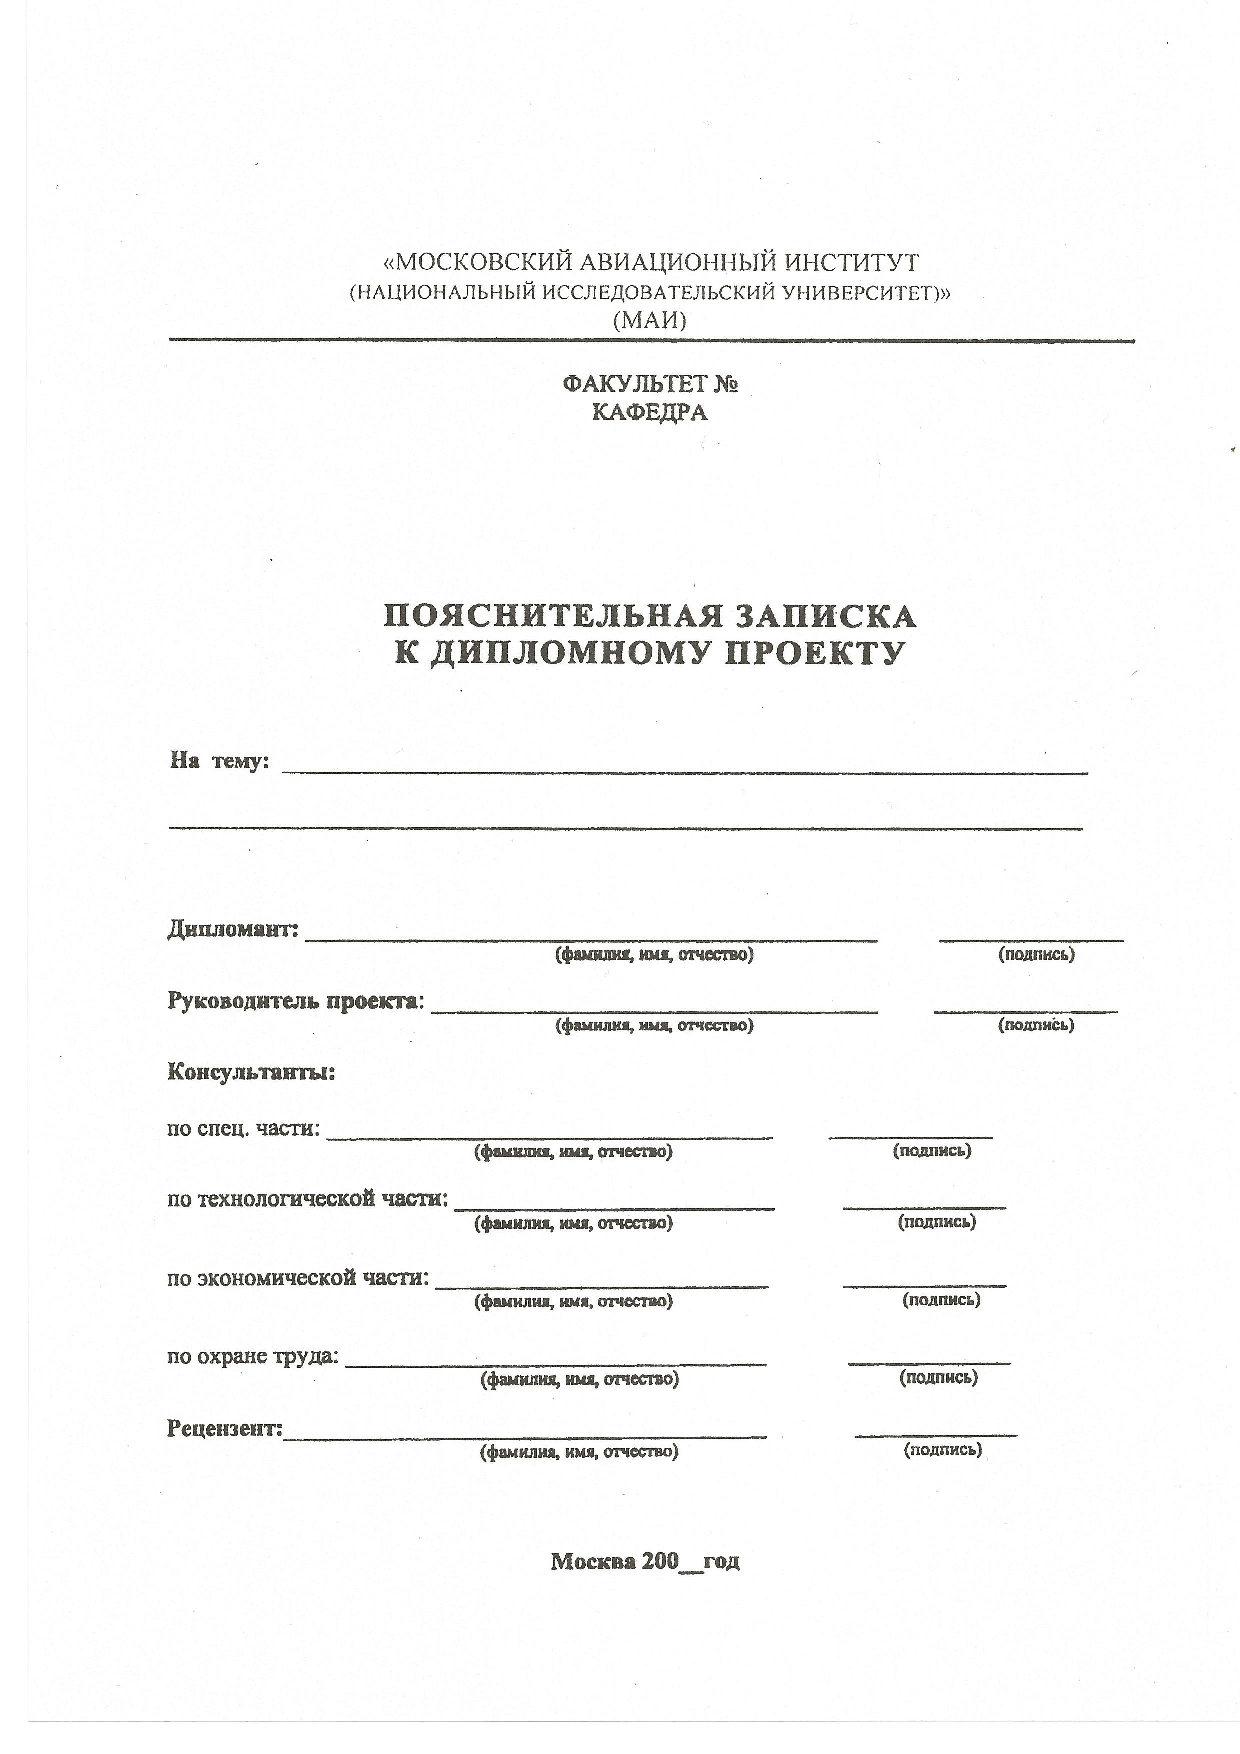
\includepdf[pages={1}]{title.pdf} % титульник
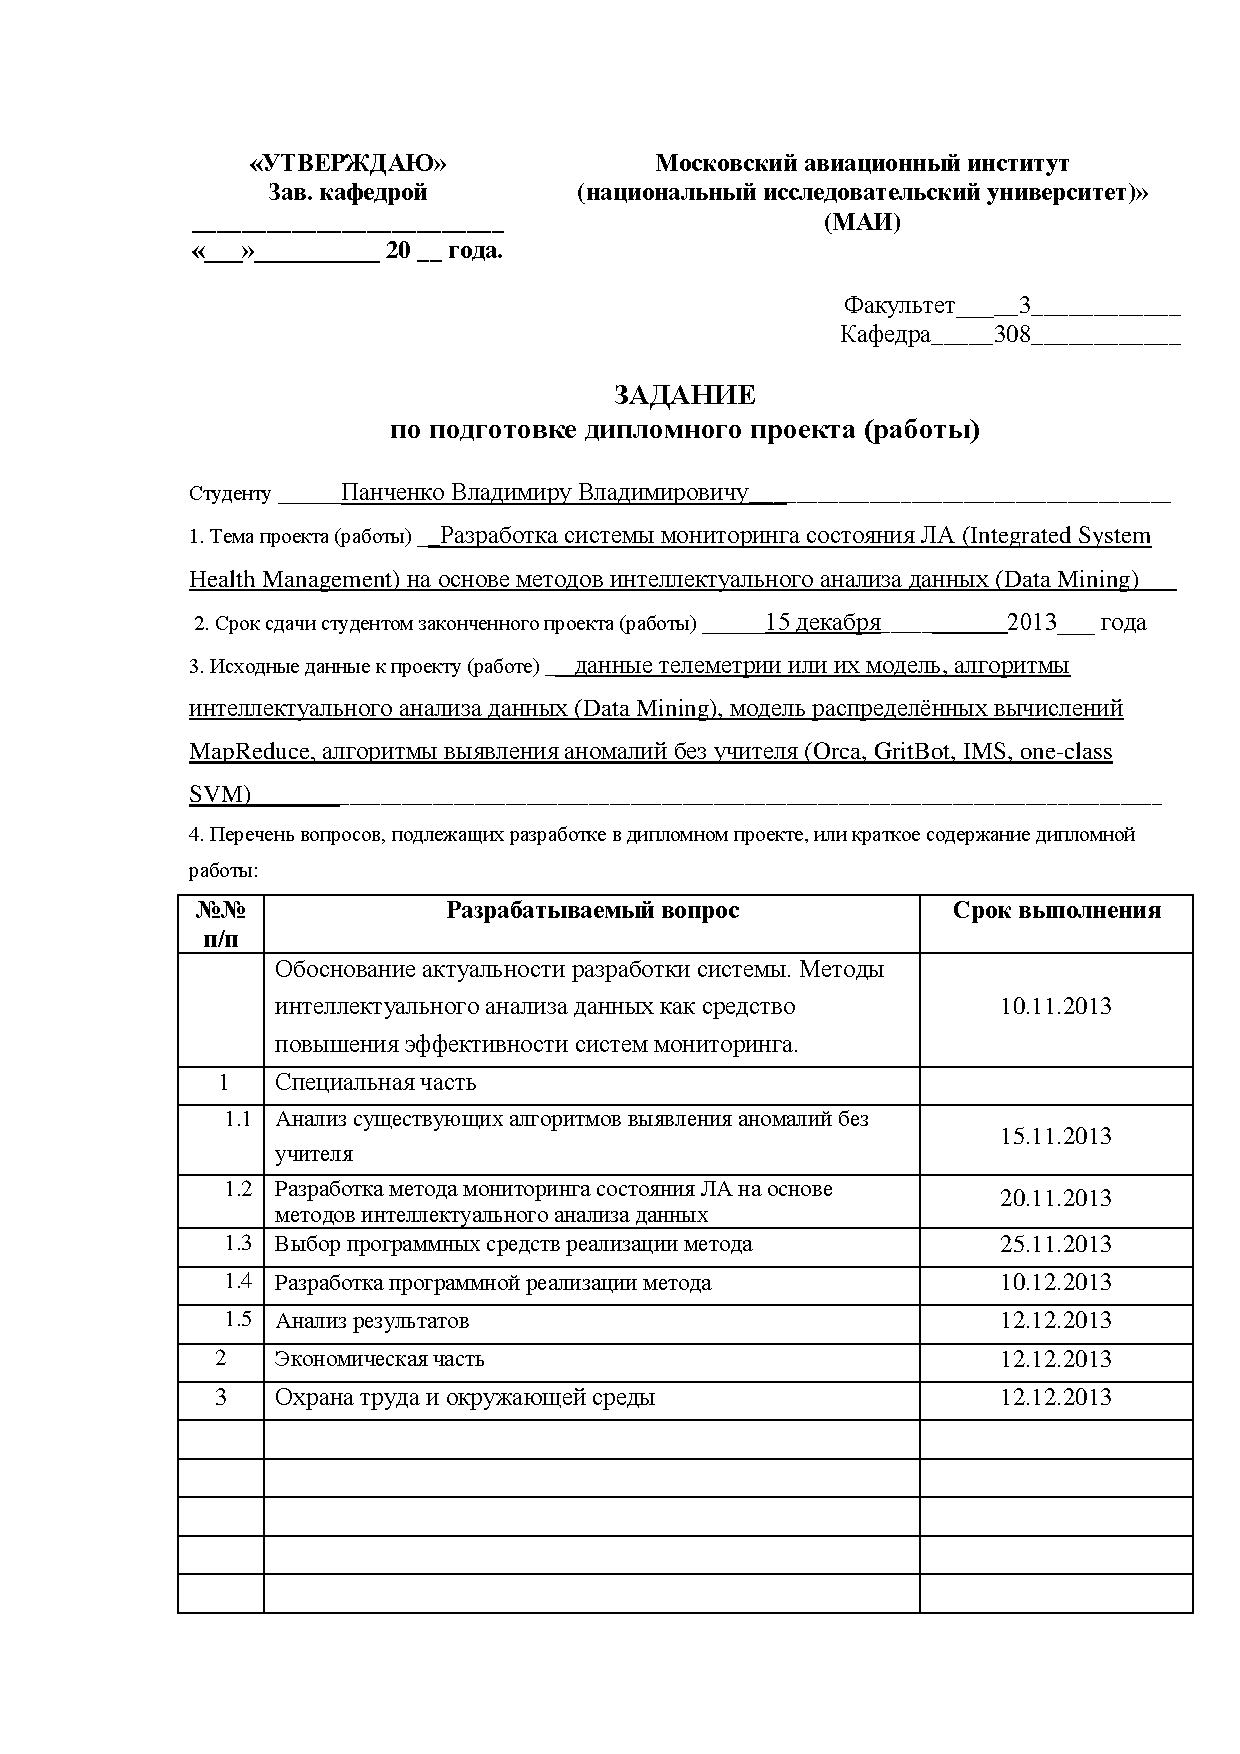
\includepdf[pages={1,2}]{assignment.pdf} % задание
\setcounter{page}{3} % начать нумерацию страниц с №3
\tableofcontents
\newcommand{\thesistitle}{Разработка системы мониторинга состояния ЛА (Integrated System Health Management) на основе методов интеллектуального анализа данных (Data Mining)}
\newcommand{\thesisauthor}{Панченко В.В.}
\newcommand{\thesiskeywords}{Data Mining, поиск аномалий, кластеризация, Integrated System Health Monitoring}

\protect\spchapter*{\MakeUppercase{Реферат}}
\sloppy
{
\thesisauthor\ \MakeUppercase{\thesistitle}, дипломная работа: \pagecount~с., \total{figurecount}~рис., \total{tablecount}~табл., \total{refcount}~ист., \total{appendixcount}~прил.

Ключевые слова: \MakeUppercase{\thesiskeywords}
}
\spchapter{Введение}
Пробелы или табуляция? Двойные или одинарные кавычки? Открывать фигурную скобку с новой строки или в «египетском» стиле? Вокруг этих соглашений оформления исходников постоянно бурлят священные войны. Впрочем, мало кто решается спорить с тем, что если работаешь в команде, то писать надо так, как в этой команде принято, или хотя бы переформатировать свой код в принятом стиле перед коммитом. В конце концов, если бы у какого-то стиля было абсолютно решающее преимущество перед другим, то и споров бы не возникало, так что, возможно, самое мудрое решение~--- делать как все. 
\chapter{Специальная часть}
\chapter{Специальная часть}
\chapter{Охрана труда и окружающей среды}
\section{Анализ условий труда}
\subsection{Обеспечение условий труда в отделе разработки программного обеспечения}
Дипломная работа посвящена разработке системы мониторинга состояния ЛА на основе алгоритмов интеллектуального анализа данных. Разработка производится на персональном компьютере и предполагает длительное пребывание за ним инженера.

Применение персонального компьютера освобождает человека от непроизводительной работы, связанной с обработкой информации, изменяет характер его труда. Однако при этом увеличивается доля умственного и нервно-напряженного труда, возрастает психоэмоциональная нагрузка. При значительной трудовой нагрузке, нерациональной организации работы и неблагоприятных факторах производственной среды быстро снижается работоспособность операторов, уменьшается производительность труда и ухудшается качество работы, может развиться перенапряжение,~а в отдельных случаях возникнуть срыв трудовой деятельности~--- дистресс.

В данном разделе проводится анализ условий труда в отделе разработки информационных систем с целью обеспечения безопасности и удобства, требуемых для работы инженера.

\subsection{Характеристика помещения}
Помещение находится в здании Московского Авиационного Института и представляет собой кафедральную лабораторию со следующими размерами:
\begin{itemize}
	\item длина~6~м;
	\item ширина~4~м;
	\item высота~3.5~м.
\end{itemize}

Площадь: $6\times4 = 24$~м\textsuperscript{2}.

Объём: $6\times4\times3,5 = 84$~м\textsuperscript{3}.

Количество рабочих мест~---~4.

Количество одновременно находящихся в помещении сотрудников не превышает~4 человек.

План помещения приведён на рисунке~\ref{fig:labourprotection:room_plan}.
\begin{figure}[h]
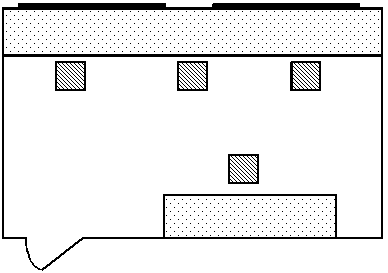
\includegraphics[width=0.6\textwidth, keepaspectratio]{plan}
\caption{План помещения}\label{fig:labourprotection:room_plan}
\end{figure}

Нормативные требования к площади и объёму рабочих мест определены в \cite{SanPin2_2_2}:
\begin{itemize}
	\item площадь на одно рабочее место с ВДТ или ПЭВМ для взрослых пользователей должна составлять не~менее~6~м\textsuperscript{2};
	\item объём~---~не~менее~20~м\textsuperscript{3}.
\end{itemize}

Фактические значения на каждого сотрудника:
\begin{itemize}
	\item площадь: $24/4 = 6$~м\textsuperscript{2};
	\item объём: $84/4 = 21$~м\textsuperscript{3}.
\end{itemize}

Данные значения показывают, что кафедральная лаборатория полностью соответствует установленным нормам.

В помещении имеются 2 оконных проёма высотой 1,6~м и шириной 2,3~м, которые выходят на юго-запад.

Искусственное освещение представляет собой 6~светильников, расположенных параллельно окнам в~2~ряда.

\subsection{Характеристика производственного процесса}
Разработка программного обеспечения производится на ПЭВМ с подключенными к ней периферийными устройствами.

\subsection{Характеристика используемого оборудования}
В процессе разработки используется следующее оборудование:
\begin{enumerate}
	\item{ПЭВМ:}
		\begin{enumerate}
			\item{процессор Intel Core i5 3,60 ГГц;}
			\item{оперативная память 8 Гб;}
			\item{жёсткий диск 1 Tб;}
			\item{напряжение питания 220 В.}
		\end{enumerate}
	\item{ЖК монитор с диагональю 23 дюйма (58,42) ASUS VX239H:}
		\begin{enumerate}
			\item{частота 75 Гц;}
			\item{яркость 250 кд/м\textsuperscript{2};}
			\item{динамическая контрастность 8 000 000 : 1;}
			\item{напряжение питания 220 В.}
		\end{enumerate}
	\item{Клавиатура Logitech K330;}
	\item{Мышь A7Tech X;}
	\item{Принтер HP LaserJet 1005M:}
		\begin{enumerate}
			\item{напряжение питания 220 В.}
		\end{enumerate}
\end{enumerate}

\subsection{Санитарно-гигиенические факторы}

\subsubsection{Микроклимат помещения}
Микроклимат в рабочем помещении должен соответствовать \cite{GOST12_1_005}.

Согласно \cite{GOST12_1_005}, работа разработчика ПО относится к категории «Легкая~–~Iа», т.к. лёгкие физические работы~--- работы с расходом энергии не более 150 ккал (174 Вт), а категория Iа подразумевает энергозатраты до 120~ккал/ч~(139 Вт).

Рабочее место разработчика ПО является постоянным, т.к. он находится на нём большую часть рабочего времени (более~50\%).

Нормативные и фактические значения для категории работ «Легкая~–~Iа», лёгкие физические работы~--–~работы с расходом энергии не более 150~ккал (174~Вт). Категория Iа подразумевает энергозатраты до 120~ккал/ч (139~Вт).

Рабочее место разработчика модели является постоянным, т.к. он находится на нём большую часть рабочего времени (более 50\%).

Нормативные и фактические значения для категории работ «Легкая – Iа» и постоянного рабочего места приведены в таблице~\ref{tab:labourprotection:microclimat}.

\begin{table}[h]
\caption{Значения характеристик микроклимата помещения}
\label{tab:labourprotection:microclimat}
\nohyphenation

\begin{tabular}{|C{84pt}|C{178.25pt}|C{101.1pt}|C{110pt}|}
\hline
 & Температура, \textdegree C & Относительная влажность, \% & Скорость движения, м/с \\
\hline
Допустимые значения & 22--24~–-- Холодный период \linebreak 23--25~--– Теплый период & 40--60 & 0.1 \\
\hline
Фактические значения & 22--24~–-- Холодный период \linebreak 25--30~--– Теплый период & 45--55 & <0.1 \\
\hline
\end{tabular}
\end{table}

Фактические значения параметров микроклимата данного помещения удовлетворяют допустимым значениям для холодного периода года. Во время теплого периода в помещении может преобладать повышенная температура из-за отсутствия кондиционера, который бы мог её регулировать.

\subsubsection{Производственное освещение}
Освещённость регламентируется~\cite{SNiP23_05_95}.

Наименьший размер объекта различения в работе инженера составляет 0.3 мм. Объектом является символ, выводимый на экран монитора (наименьшим символом является точка). Зрительная работа относится к III разряду --- высокая точность (наименьший размер объекта различения от 0.3 до 0.5~мм).

Контраст объекта с фоном средний, фон светлый, что соответствует подразряду~б разряда III.

Требования к освещению помещений промышленных предприятий для подразряда~б разряда III:
\begin{itemize}
	\item При системе комбинированного освещения освещенность равна: всего --- 1000 лк, в т.ч. от общего --- 200 лк;
	\item При системе общего освещения освещённость равна 300 лк.
\end{itemize}

Система освещения в комнате общая, состоящая из 6 потолочных светильников ЛПО 46, в каждом из которых установлены 4 люминесцентные лампы ЛТБ мощностью 20 Вт и световым потоком 1100 лм. Светильники расположены в два ряда параллельно окнам. Фактическая освещенность составляет 275 лк, что полностью удовлетворяет нормативным значениям~\cite{SNiP23_05_95}.

\subsubsection{Шум}
Источники шума в данном помещении: охлаждающие системы ПЭВМ (охлаждение процессоров).

Уровни шума на рабочих местах инженера ПЭВМ должны соответствовать~\cite{GOST12_1_003}.

Допустимые значения уровня шума при проектировании и программировании на рабочих местах в помещениях – проектно-конструкторских бюро; расчётчиков, программистов вычислительных машин, в лабораториях для теоретических работ и обработки данных: не более  50 дБА.

Фактические значения уровня шума: не более 45 дБА, что подтверждается расчётами в пункте~\ref{sec:labourprotection:calc}.

Согласно~\cite{GOST12_1_003}, значения уровня шума на рабочем месте удовлетворяют установленным требованиям.

\subsubsection{Электромагнитное излучение}
Во время работы ПЭВМ возникают электромагнитные поля, которые оказывают негативное влияние на организм человека.

Источниками электромагнитных полей на рабочем месте инженера являются системные блоки. Современные корпуса системных блоков ПЭВМ позволяют значительно ослабить излучения его элементов. Благодаря существующим достаточно строгим стандартам дозы рентгеновского излучения от современных мониторов и системных блоков не опасны для пользователей.

Документом, регламентирующим уровень электромагнитного излучения для ПЭВМ, является~\cite{SanPin2_2_2}.

Согласно ему, напряжённости электрических и магнитных полей, энергетической нагрузки в течение рабочего дня не должны превышать значений, указанных в таблице~\ref{tab:labourprotection:emradiation}.

\begin{table}[h]
\caption{Предельные значения электромагнитного излучения.}
\label{tab:labourprotection:emradiation}
\nohyphenation

\begin{tabular}{|C{213.35pt}|C{87.35pt}|C{84.4pt}|C{83.4pt}|}
\hline
\multirow{2}{\hsize}{\centering{Параметр}} & \multicolumn{3}{C{255.15pt}|}{Предельные значения в диапазонах частот, МГц} \\
\cline{2-4}
 & от 0.06 до 3 & св. 3 до 30 & св. 30 до 300 \\
\hline
Е\textsubscript*{ПД}, В/м & 500 & 300 & 80 \\
\hline
Н\textsubscript*{ПД}, А/м & 50 & --- & --- \\
\hline
ЭН\textsubscript*{Е\textsubscript*{ПД}}, (В/м)\textsuperscript{2} $\cdot$ ч & 20000 & 7000 & 800 \\
\hline
ЭН\textsubscript*{Н\textsubscript*{ПД}}, (А/м)\textsuperscript{2} $\cdot$ ч & 200 & --- & --- \\
\hline
\end{tabular}
\end{table}

Монитор ASUS VX239H соответствует стандарту~\cite{TCO03}, который устанавливает следующие предельные значения электромагнитного излучения:
\begin{itemize}
	\item напряжённость электрического поля: в диапазоне 5Гц--2кГц не более 10~В/м, в диапазоне 2кГц--400кГц не более 1.0~В/м;
	\item напряжённость магнитного поля: в диапазоне 5Гц--2кГц не более 200~нТл, в диапазоне 2кГц--400кГц не более 25~нТл.
\end{itemize}

Данные характеристики полностью соответствуют требованиям~\cite{SanPin2_2_2}.

\subsection{Электроопасность}
В данном помещении используется оборудование, питающееся от сети переменного тока напряжением 220~В, частотой 50~Гц. 

Согласно~\cite{PUE7}, помещение отдела разработки ИС относится к классу помещений без повышенной опасности поражения электрическим током: это сухое помещение с непроводящими полами, с нормальной температурой воздуха и влажностью, в нем отсутствует токопроводящая пыль.

Электрооборудование в помещении представлено мониторами и системными блоками ПЭВМ. Источником электрического поражения может быть металлический корпус системного блока при пробое изоляции, т.к. имеется напряжение 220~В, а в~\cite{GOST12_1_038} допустимое напряжение и ток для аварийных режимов при времени воздействия более 1~секунды составляют 20~В и 6~мА.

\subsection{Пожароопасность}
В данном помещении имеются твердые горючие и  трудногорючие веще-ства и материалы (книги, документы, деревянная мебель, оргтехника и т.д.), которые при взаимодействии с огнем будут гореть без взрыва. Также источником возгорания может быть электрическая проводка.

Согласно~\cite{GOST12_1_004}, данное помещение относится к классу Б и является пожароопасным.

\subsection{Эргономические факторы}
Требования к организации рабочих мест пользователей ПЭВМ изложены в~\cite{SanPin2_2_2}. 

Согласно~\cite{SanPin2_2_2}, расстояние между рабочими столами с мониторами (в направлении тыла поверхности одного монитора и экрана другого монитора) должно быть не менее 2~м, а расстояние между боковыми поверхностями мониторов не менее 1.2~м.

Фактические значения (см. рисунок~\ref{fig:labourprotection:room_plan}):
\begin{itemize}
	\item расстояние между рабочими столами 2.1--2.5~м;
	\item расстояние между боковыми поверхностями мониторов 2.1-2.3~м.
\end{itemize}

Таким образом, размещение рабочих столов полностью соответствуют требованиям~\cite{SanPin2_2_2}.

В помещении используется специальный стол~--– рабочая поверхность, изготовленная на заказ по выбранным заказчиком параметрам. Ее характеристики и нормативные значения указаны в таблице~\ref{tab:labourprotection:desktop}.

\begin{table}[h]
\caption{Характеристики используемого рабочего стола}
\label{tab:labourprotection:desktop}
\nohyphenation

\begin{tabular}{|C{225.9pt}|C{125.05pt}|C{114.85pt}|}
\hline
Наименование параметра & Нормативное значение~\cite{SanPin2_2_2}, мм & Фактическое значение, мм \\
\hline
Ширина рабочей поверхности & не менее 500  & 1200--2000 \\
\hline
Глубина рабочей поверхности & не менее 800 & 800 \\
\hline
Высота рабочей поверхности & не менее 725 & 800 \\
\hline
Пространство для ног высотой & не менее 600 & 600 \\
\hline
Глубина на уровне колен & не менее 450 & 450 \\
\hline
Глубина на уровне вытянутых ног & не менее 650 & 650 \\
\hline
\end{tabular}
\end{table}

Параметры стола полностью соответствуют требованиям~\cite{SanPin2_2_2}.

В помещении используется офисное кресло БЮРОКРАТ Ch-G318AXN. Его характеристики и нормативные размеры указаны в таблице~\ref{tab:labourprotection:chair}.

\begin{longtable}{|C{197.55pt}|C{153.4pt}|C{114.85pt}|}
\caption{Характеристики используемого офисного кресла}
\label{tab:labourprotection:chair}
\\
\hline
Наименование параметра & Нормативное значение~\cite{SanPin2_2_2} & Фактическое значение \\
\endhead
\hline
Ширина и глубина поверхности сиденья & не менее 400 мм & 420 мм \\
\hline
Регулировка высоты поверхности сиденья  & 400--550 мм & 440--570 мм \\
\hline
Регулировка углов наклона сиденья & вперед до 15\textdegree и назад до 5\textdegree & вперед до 15\textdegree и назад до 5\textdegree \\
\hline
Высота опорной поверхности спинки & 300 ± 20 мм & 310 мм \\
\hline
Ширина опорной поверхности спинки & не менее 380 мм & 380 мм \\
\hline
Радиус кривизны горизонтальной плоскости опорной поверхности спинки & 400 мм & 400 мм \\
\hline
Угол наклона спинки в вертикальной плоскости & ± 30\textdegree & ± 30\textdegree \\
\hline
Регулировка расстояния спинки от переднего края сиденья & 260--400 мм & 260--450 мм \\
\hline
Стационарные или съёмные подлокотники & длина не менее 250 мм \linebreak ширина 50--70 мм & длина 250 мм \linebreak ширина 60 мм \\
\hline
Регулировка подлокотников по высоте над сиденьем & 230 ± 30 мм & Нет \\
\hline
Регулировка внутреннего расстояния между подлокотниками & 350--500 мм & 420--500 мм \\
\hline
\end{longtable}

Параметры стула частично не соответствуют требованиям \cite{SanPin2_2_2}: в данном рабочем кресле отсутствует регулировка подлокотников по высоте над сидением.

\subsection{Психофизиологические факторы}
Факторами, оказывающими влияние на внимательность инженера и его производительность труда, в условиях его рабочего места являются:
\begin{itemize}
	\item визуальные характеристики монитора (его яркость, контрастность, разрешение, частота обновления); 
	\item напряженность работы; 
	\item количество обрабатываемой информации –-- плотность воспринимаемых сигналов.
\end{itemize}

Используется ЖК монитор ASUS VX239H. Его фактические характеристики и нормативные значения~\cite{SanPin2_2_2} приведены в таблице~\ref{tab:labourprotection:display}.

\begin{table}[h]
\caption{Характеристики используемого ЖК монитора}
\label{tab:labourprotection:display}
\nohyphenation

\begin{tabular}{|C{178.9pt}|C{152.25pt}|C{158.9pt}|}
\hline
Наименование фактора & Действительное значение & Нормативное значение~\cite{SanPin2_2_2} \\
\hline
Размер экрана по диагонали & 58,42 см & не менее 31 см \\
\hline
Удалённость экрана & 60 см & не менее 50 см \\
\hline
Частота обновления изображения & 75 Гц & не менее 75 Гц \\
\hline
Контрастность & 8 000 000:1 & не менее 3:1 \\
\hline
Яркость знака & 250 кд/м2 & не менее 35 кд/м2 \\
\hline
\end{tabular}
\end{table}

Характеристики монитора полностью соответствуют требованиям~\cite{SanPin2_2_2}.

Напряженность работы на основании данных таблицы классов условий труда по показателям напряженности трудового процесса \cite{R2_2_2006} представлена в таблице~\ref{tab:labourprotection:workintensity}.

\afterpage{
\begin{longtable}{|C{165pt}|C{165pt}|C{155pt}|}
%\nohyphenation
\caption{Напряженность работы}
\label{tab:labourprotection:workintensity}
\\
\hline
Критерий & Характеристика & Напряженность трудового процесса \\
\endhead
\hline
Содержание работы & Решение сложных задач по известным алгоритмам (работа по серии инструкций) & Напряженный труд 1 степени \\
\hline
Восприятие сигналов (информации и их оценка) & Восприятие сигналов с последующей комплексной оценкой взаимосвязанных параметров & Напряженный труд 2 степени \\
\hline
Степень сложности задания & Обработка, проверка и контроль за выполнением задания & Напряженность труда средней степени \\
\hline
Характер выполняемой работы & График с возможной корректировкой & --//-- \\
\hline
Длительность сосредоточенного наблюдения (в \% от времени смены) & 26--50\% & --//-- \\
\hline
Плотность сигнала за 1 час работы & 176--300 & Напряженный труд 1 степени \\
\hline
Число объектов одновременного наблюдения & 6--10 & Напряженность труда средней степени \\
\hline
Размер объекта различения, мм, при длительном сосредоточенном наблюдении (\% времени смены) & 3--10 мм до 50\% времени & --//-- \\
\hline
Степень ответственности & Ответственность за качество конечного результата & Напряженный труд 2 степени \\
\hline
Значимость ошибки & Влечет за собой дополнительные усилия в работе со стороны работника & Напряженность труда лёгкой степени \\
\hline
Продолжительность рабочего дня & 8--9 часов & Напряженность труда средней степени \\
\hline
\end{longtable}
}

Среднее значение по данным критериям соответствует средней степени напряженности труда.
\spchapter{Заключение}
*здесь должно быть заключение*
\addcontentsline{toc}{chapter}{\bibname}
\bibliography{thesis}
\end{document}